\chapter{Annexe}

\section{Introduction}
Vous entrez à présent dans la partie annexe de ce document.
Cette section complémentaire rassemble l'ensemble des ressources techniques et des informations supplémentaires indispensables à la compréhension globale du projet, mais qui auraient surchargé le corps principal du rapport.

\hypertarget{cible:Sequence}{}
\section{Diagramme de séquence}
\begin{for_you}{Diagramme de séquence Creation/modification utilisateur :}
    \begin{center}
        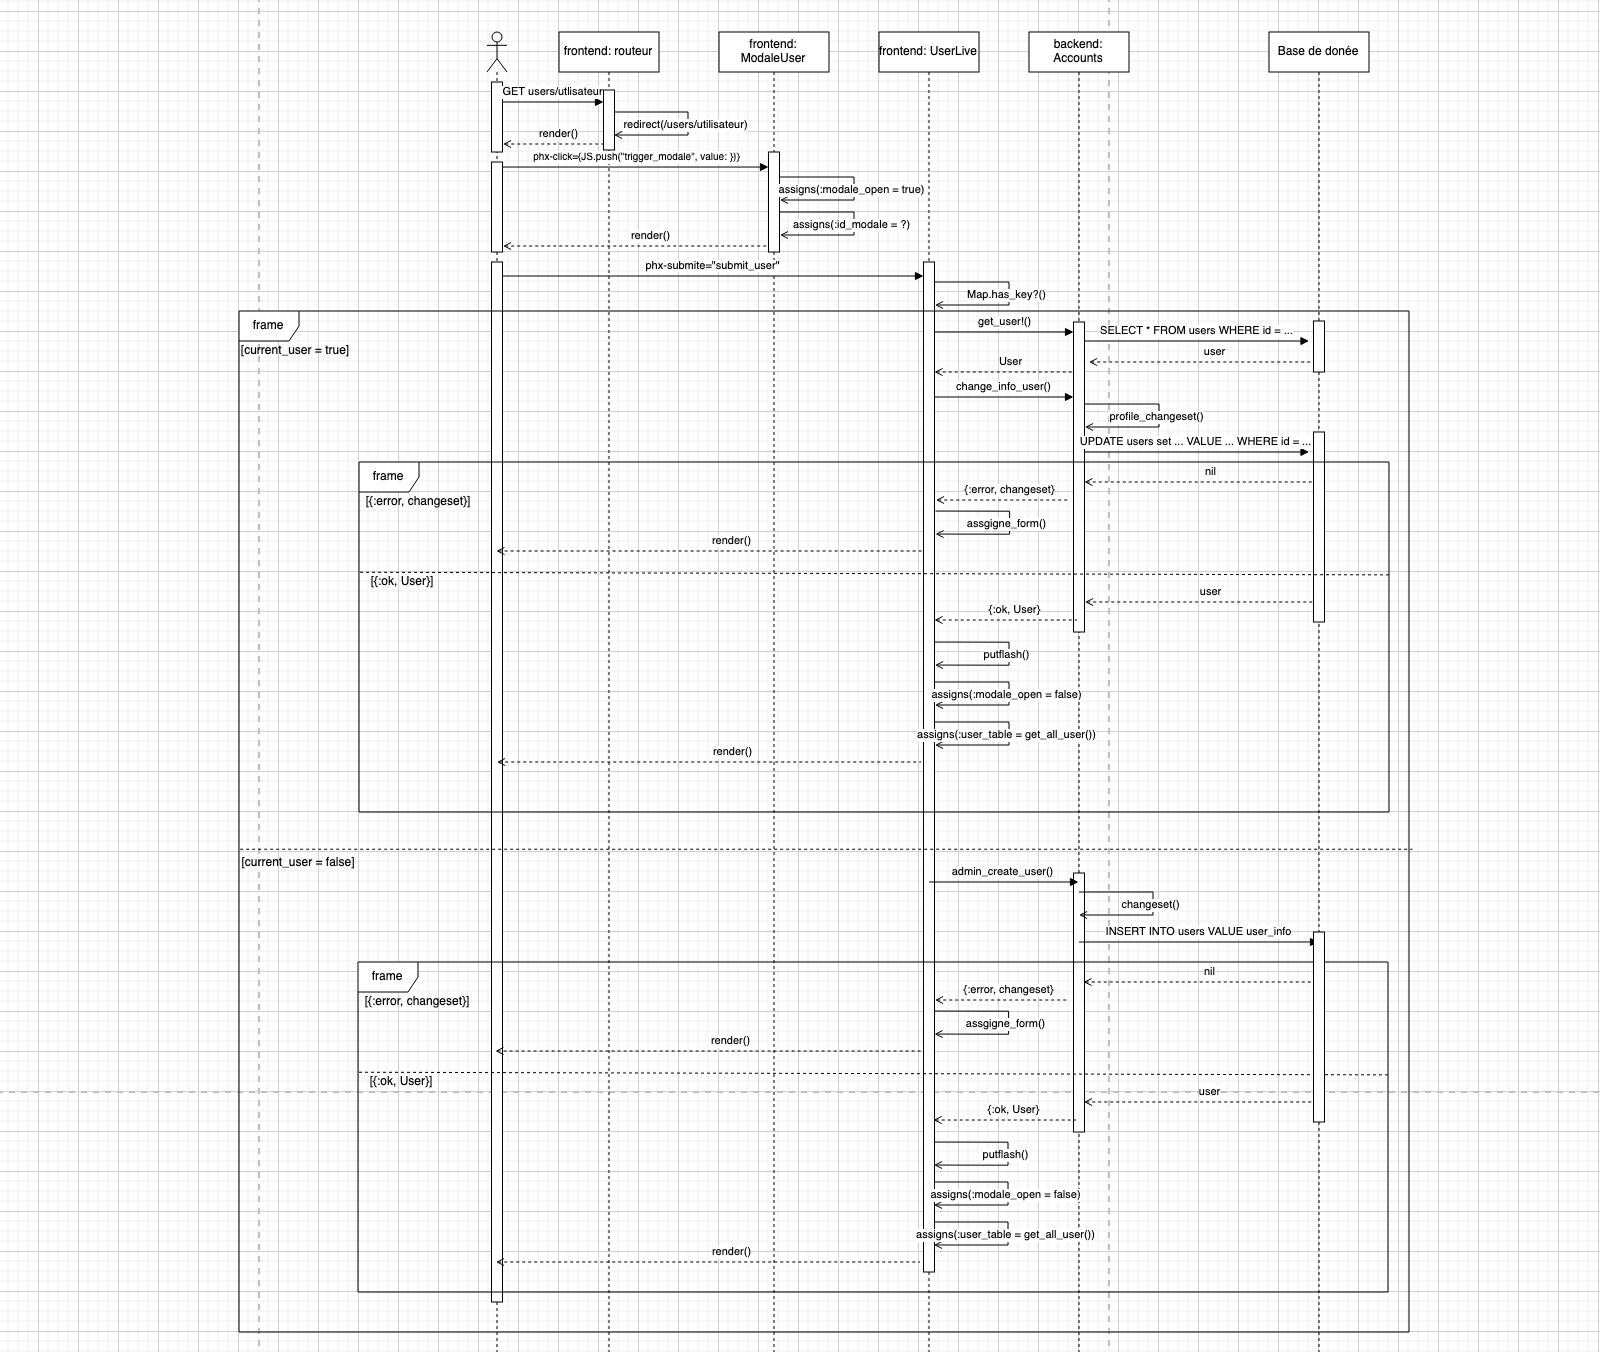
\includegraphics[width=10cm]{./assets/uml/diagramme_de_sequence_user_manager.png}
    \end{center}

    \textit{Scénario} :
    Creation/modification d'un utilisateur $\rightarrow$ verification des informations $\rightarrow$ ajoue en base.
\end{for_you}

\hypertarget{cible:Maquettage}{}
\section{Zoning}
    \begin{for_you}{Page de connexion}
        
\includegraphics[height=6.5cm]{./assets/zoning/page_de_connexion.png}
        \hfil
        
\includegraphics[height=6.5cm]{./assets/zoning/page_de_connexion_mobile.png}
    \end{for_you}

    \textbf{\newline}

    \begin{for_you}{Dashboard}
        
\includegraphics[height=7cm]{./assets/zoning/dashboard.png}
        \hfil
        
\includegraphics[height=7cm]{./assets/zoning/dashboard_mobile.png}
    \end{for_you}

\section{Wireframe}

\begin{for_you}{Page de connexion}
    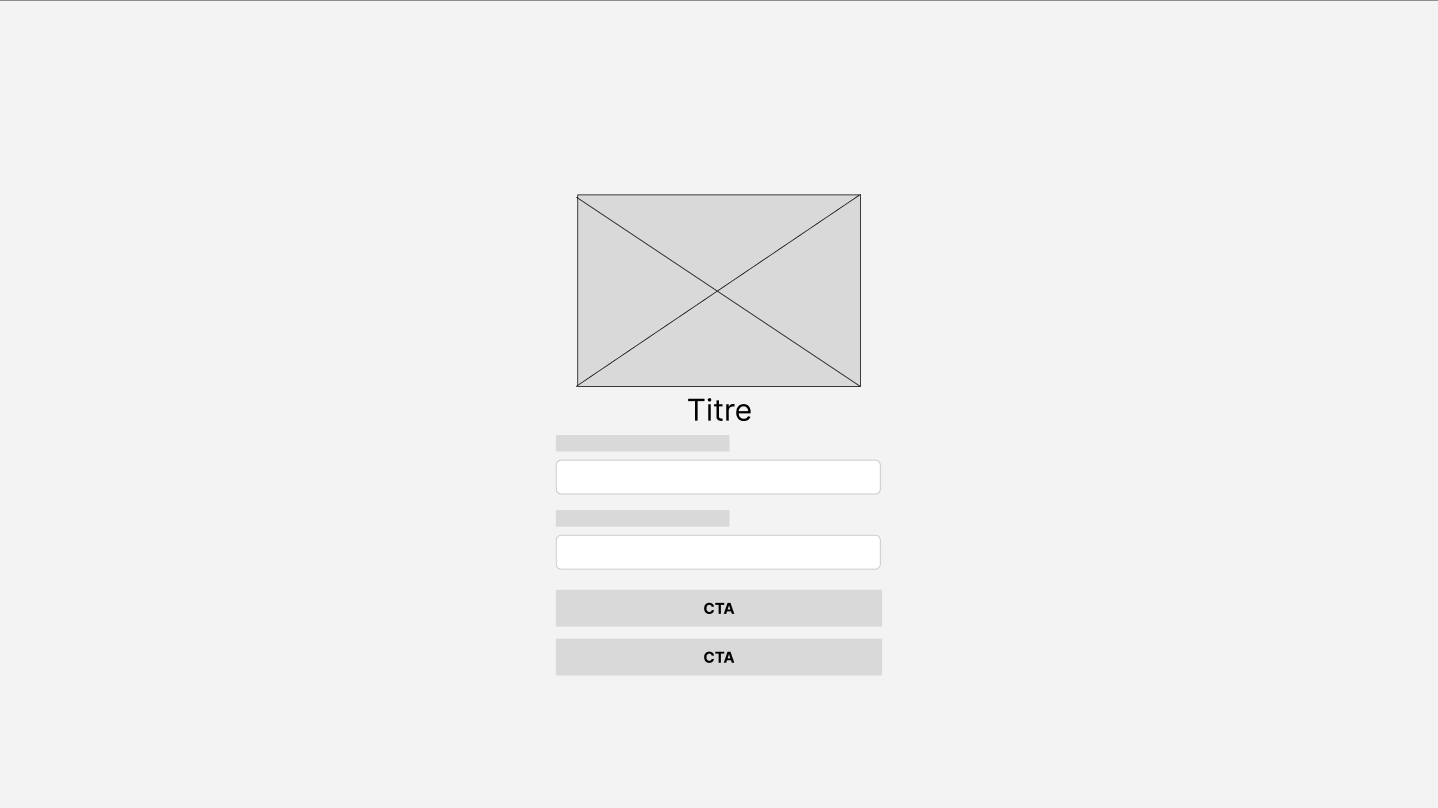
\includegraphics[height=6.5cm]{./assets/wireframe/page_de_connexion.png}
    \hfil
    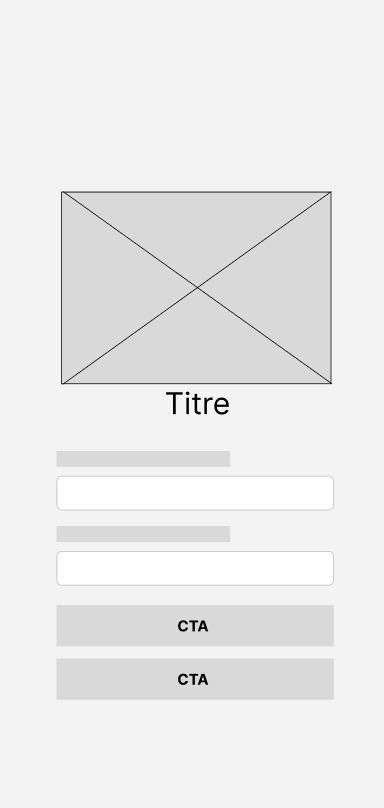
\includegraphics[height=6.5cm]{./assets/wireframe/page_de_connexion_mobile.png}
\end{for_you}

\textbf{\newline}

\begin{for_you}{Dashboard}
    
\includegraphics[height=8cm]{./assets/wireframe/dashboard.png}
    \hfil
    
\includegraphics[height=8cm]{./assets/wireframe/dashboard_mobile.png}
\end{for_you}

\textbf{\newline}

\begin{for_you}{Page de gestion d'utilisateur}
    
\includegraphics[height=8cm]{./assets/wireframe/page_utilisateur.png}
    \hfil
    
\includegraphics[height=8cm]{./assets/wireframe/page_utilisateur_mobile.png}
\end{for_you}

\textbf{\newline}

\begin{for_you}{Page de gestion badge}
    
\includegraphics[height=8cm]{./assets/wireframe/page_badge.png}
    \hfil
    
\includegraphics[height=8cm]{./assets/wireframe/page_badge_mobile.png}
\end{for_you}

\textbf{\newline}

\begin{for_you}{Page profile}
    
\includegraphics[height=8cm]{./assets/wireframe/page_profile.png}
    \hfil
    
\includegraphics[height=8cm]{./assets/wireframe/page_profile_mobile.png}
\end{for_you}

\textbf{\newline}

\begin{for_you}{Modale de création d'utilisateur}
    
\includegraphics[height=8cm]{./assets/wireframe/page_creation_utilisateur.png}
    \hfil
    
\includegraphics[height=8cm]{./assets/wireframe/page_creation_utilisateur_mobile.png}
\end{for_you}

\section{Maquettage}

\begin{for_you}{Page de connexion}
    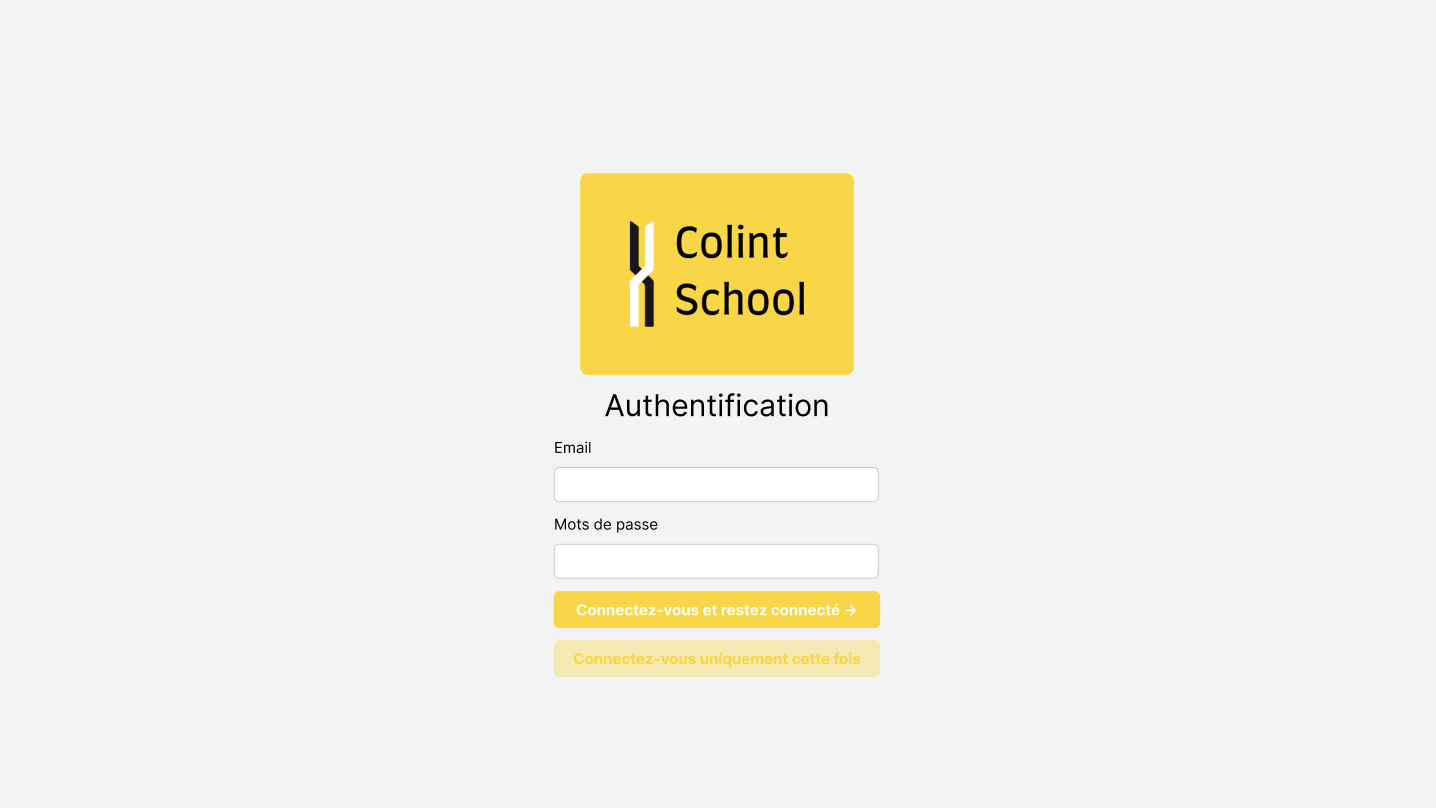
\includegraphics[height=6.5cm]{./assets/maquette/page_de_connextion.png}
    \hfil
    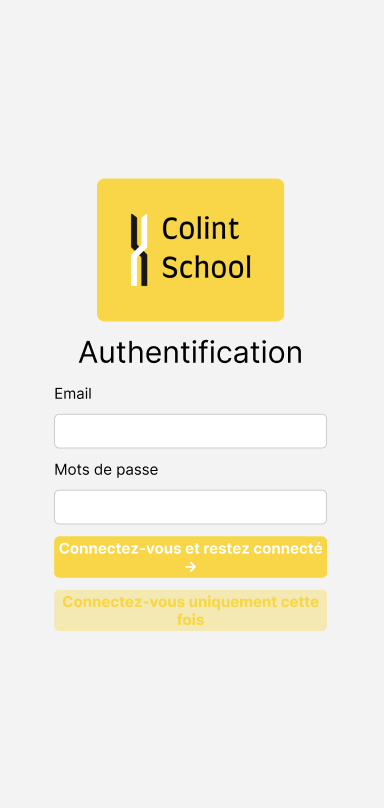
\includegraphics[height=6.5cm]{./assets/maquette/page_de_connextion_mobile.png}
\end{for_you}

\textbf{\newline}

\begin{for_you}{Dashboard}
    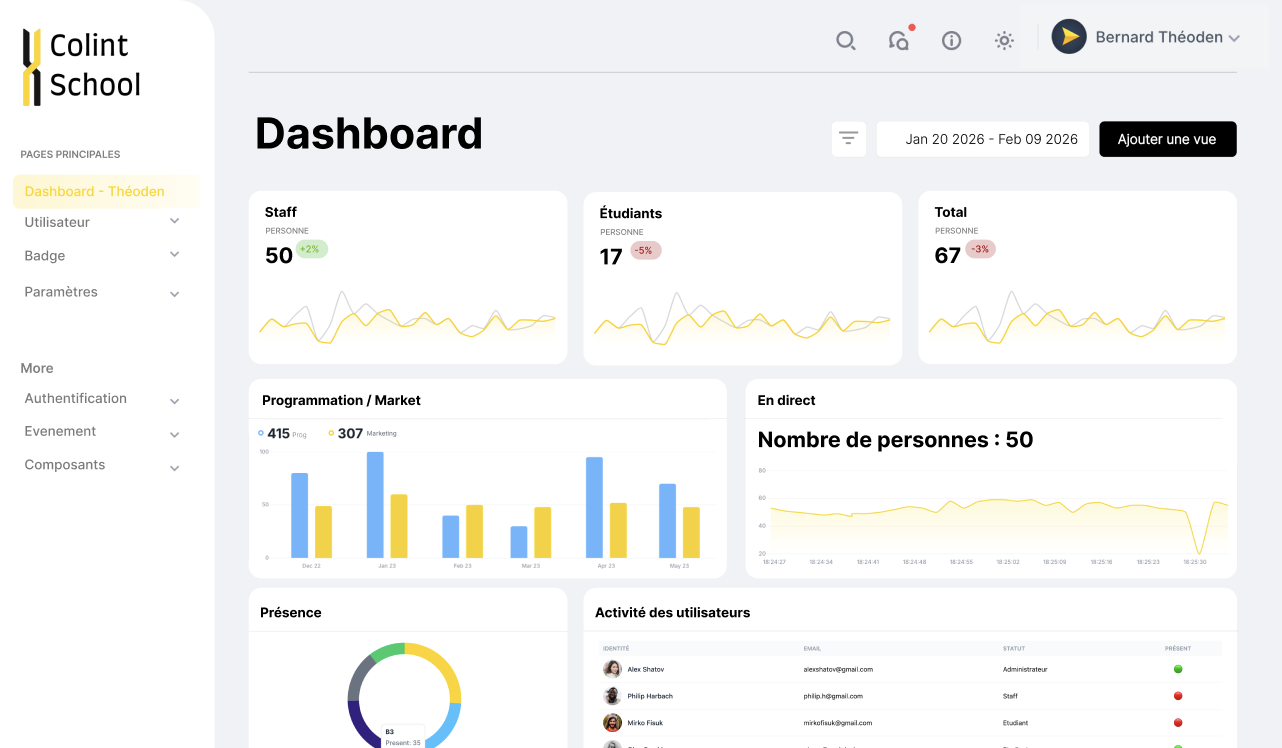
\includegraphics[height=7.5cm]{./assets/maquette/dashboard.png}
    \hfil
    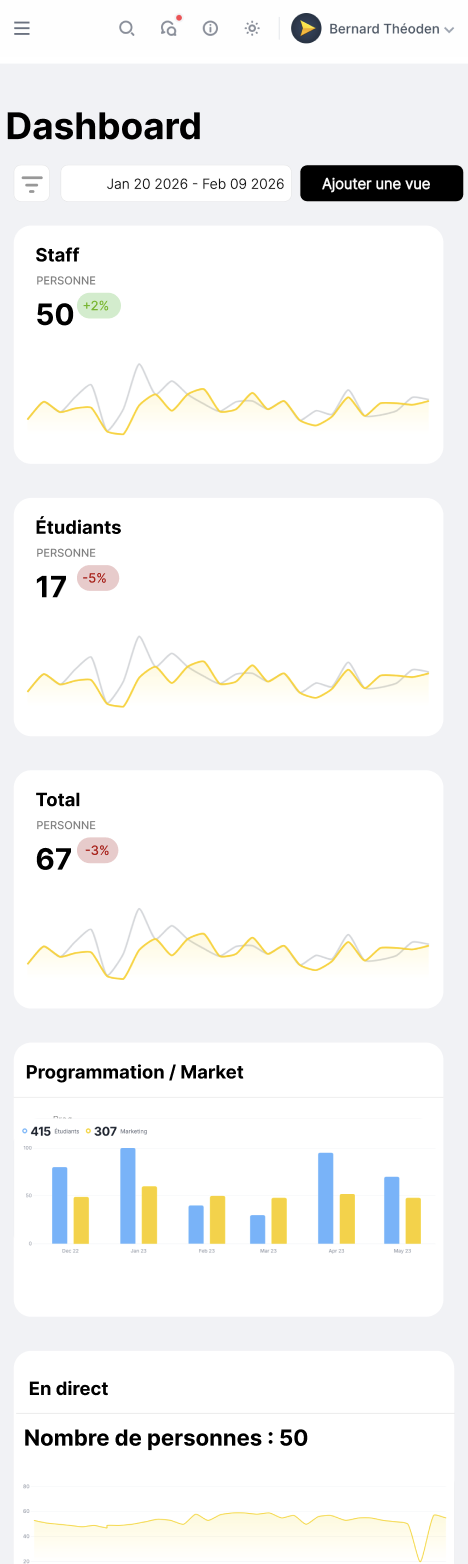
\includegraphics[height=7.5cm]{./assets/maquette/dashboard_mobile.png}
\end{for_you}

\textbf{\newline}

\begin{for_you}{Page de gestion d'utilisateur}
    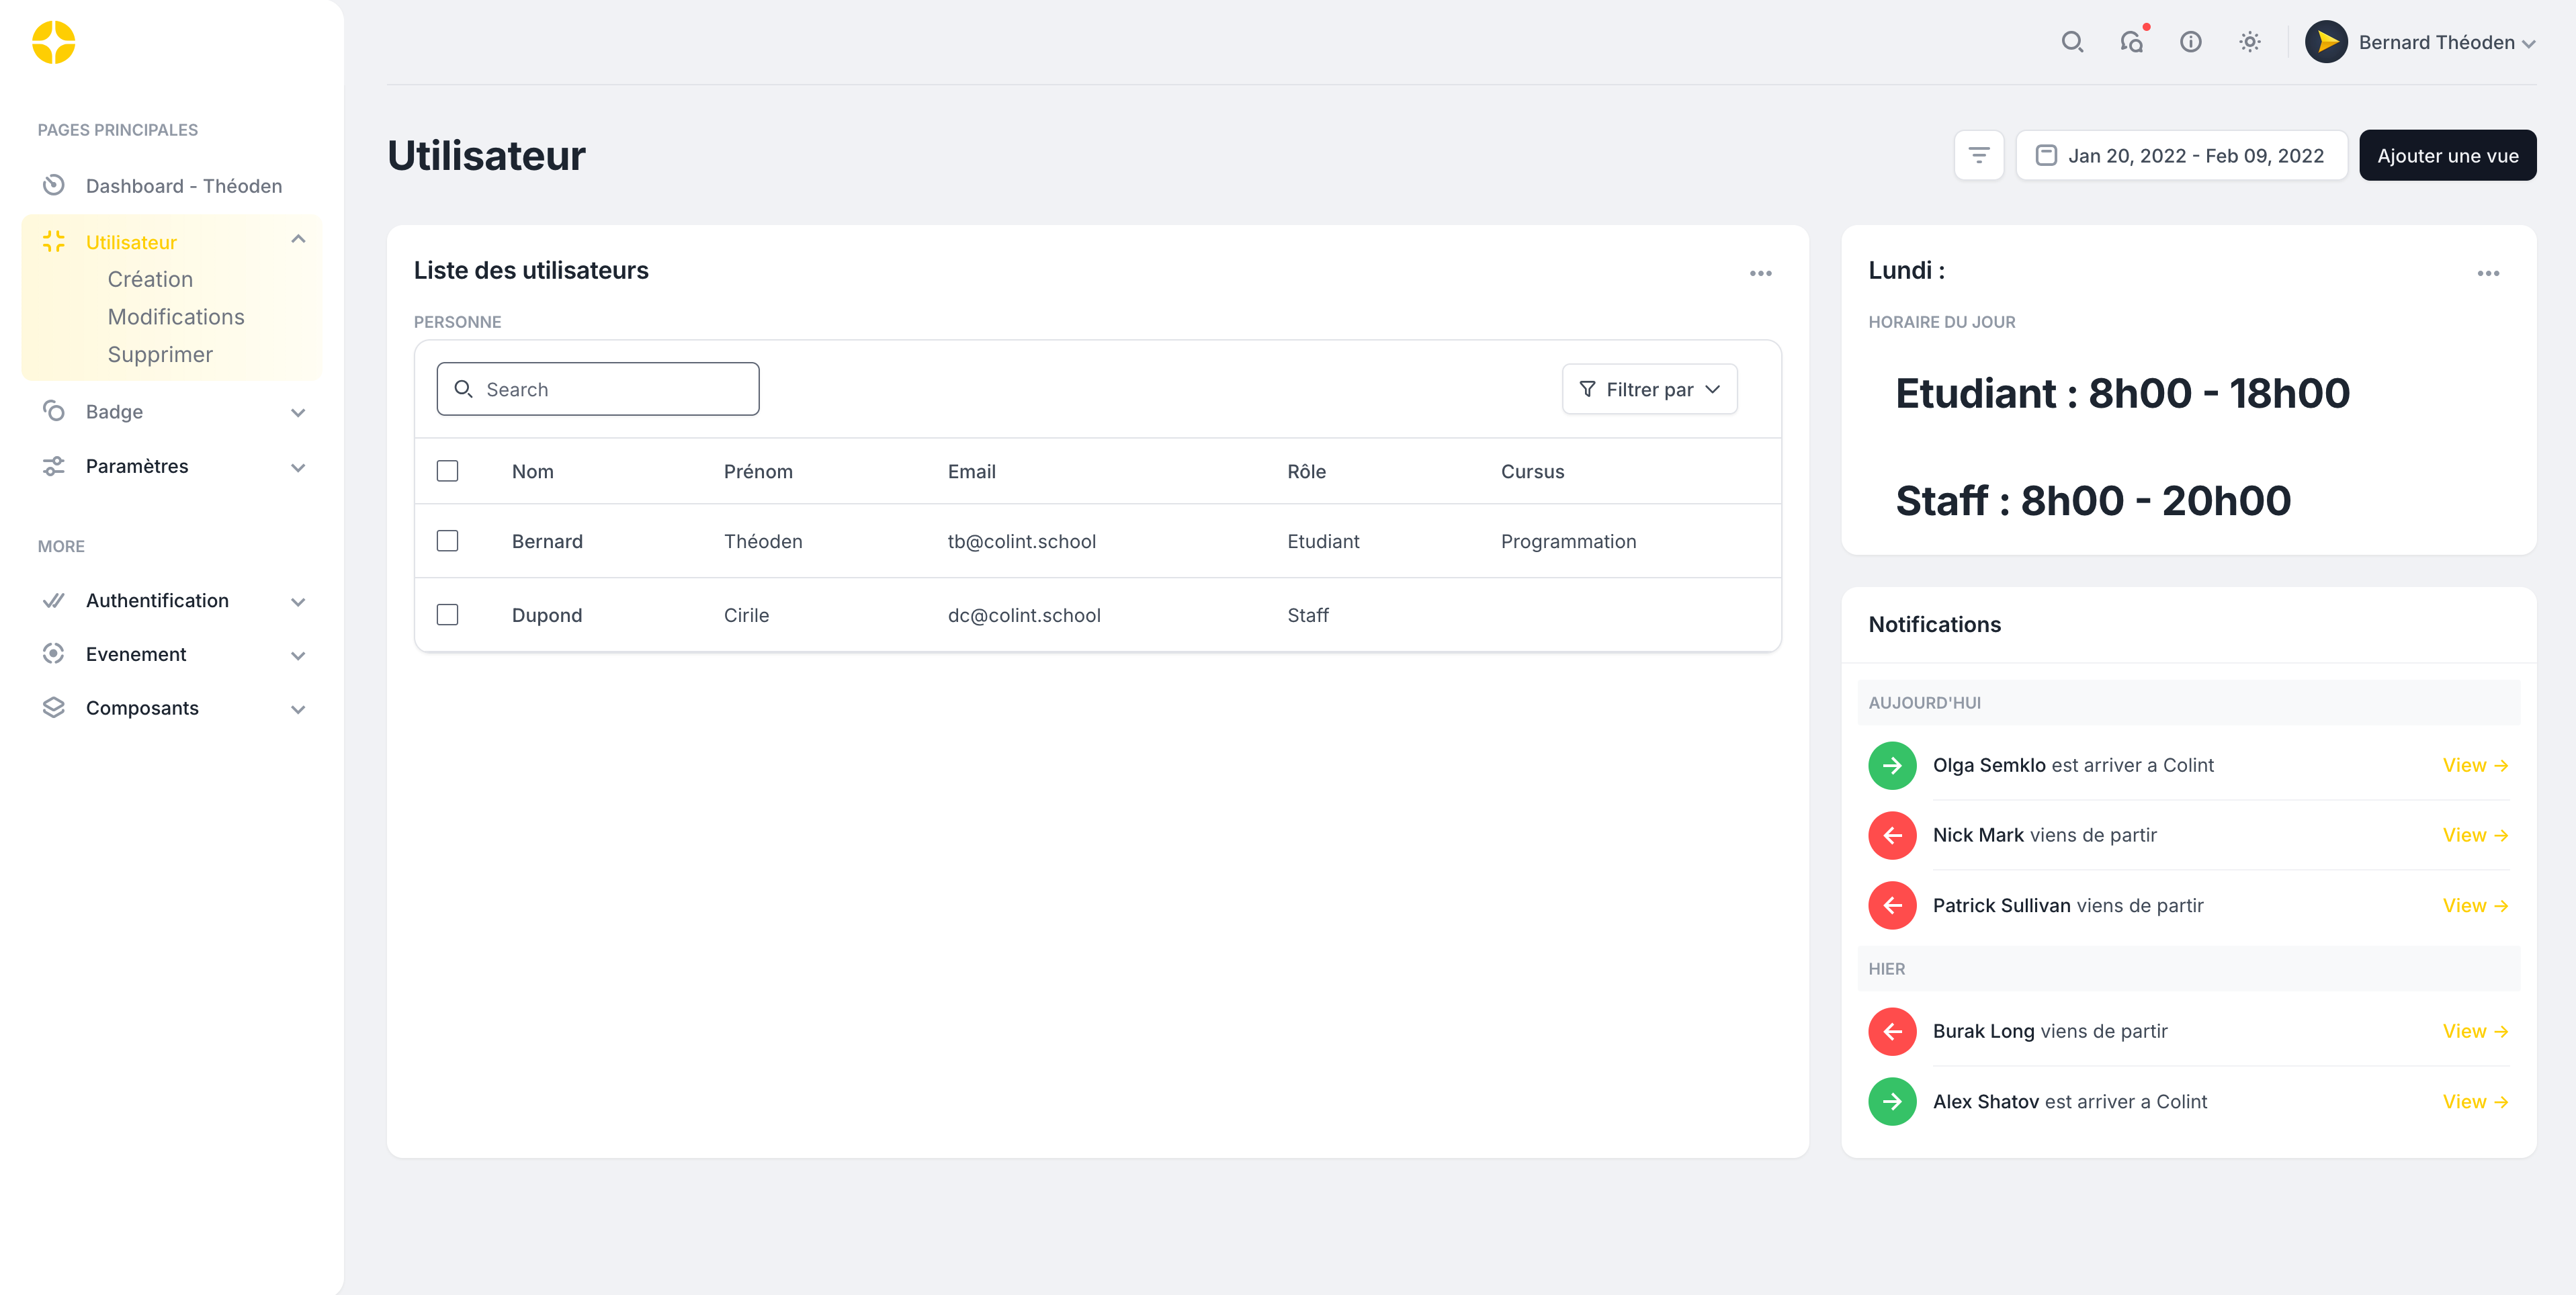
\includegraphics[height=7.2cm]{./assets/maquette/page_utilisateur.png}
    \hfil
    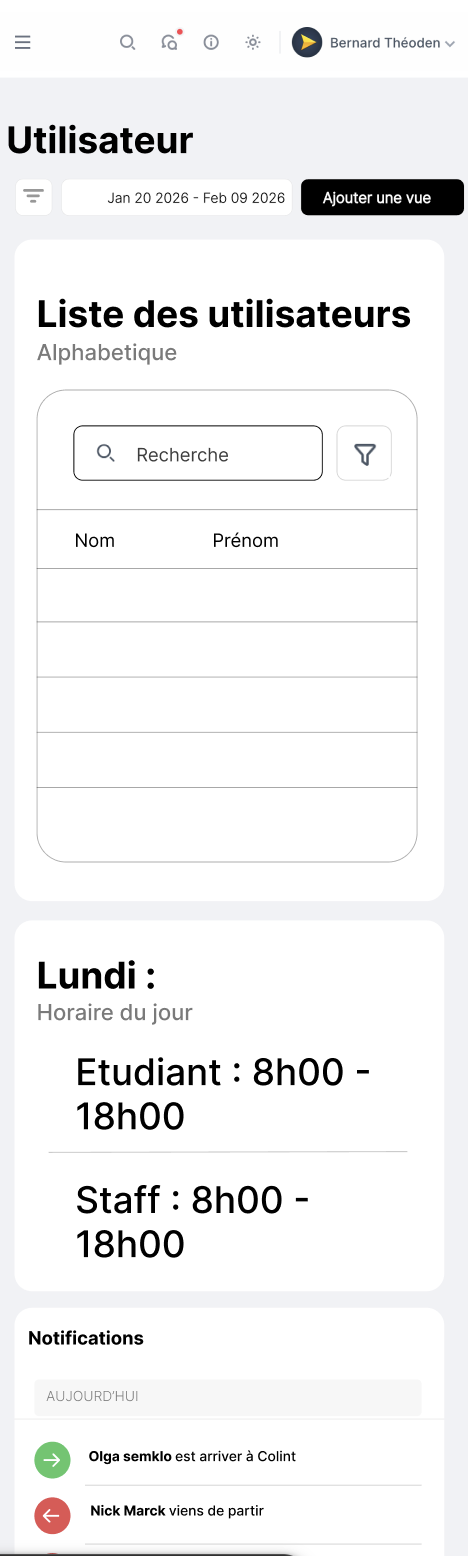
\includegraphics[height=7.2cm]{./assets/maquette/page_utilisateur_mobile.png}
\end{for_you}

\textbf{\newline}

\begin{for_you}{Page de gestion badge}
    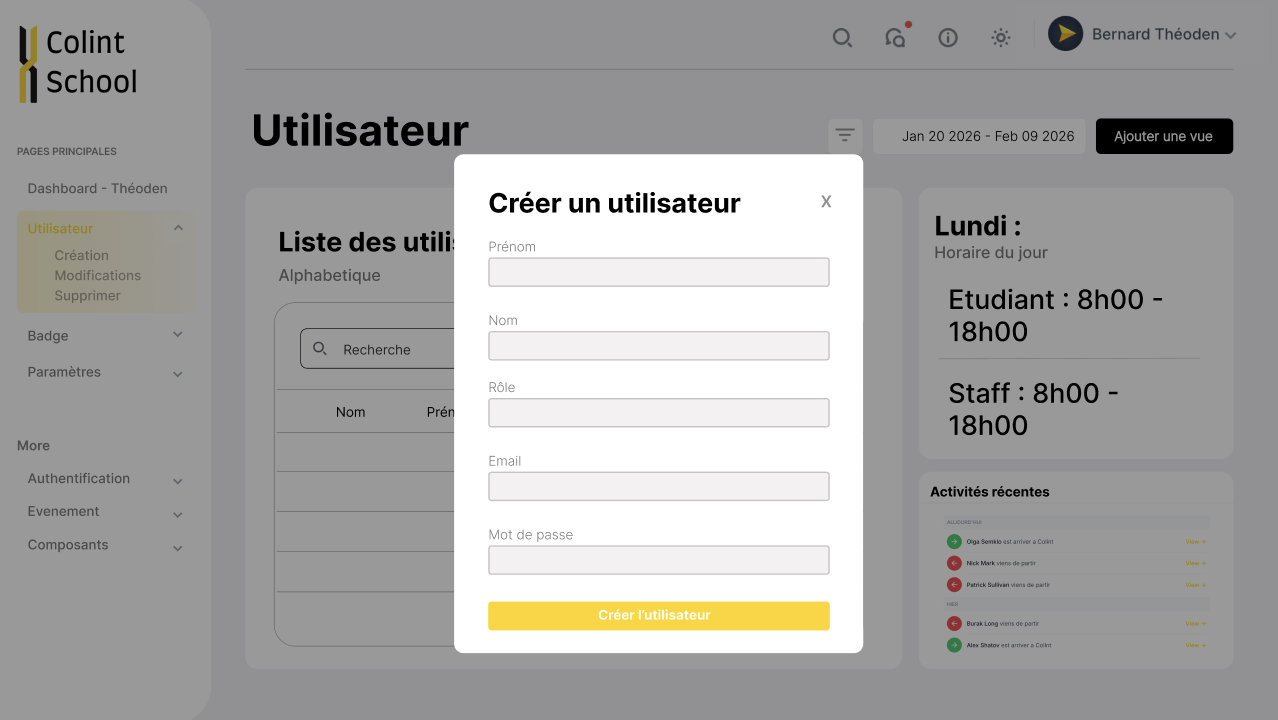
\includegraphics[height=7.2cm]{./assets/maquette/page_badge.png}
    \hfil
    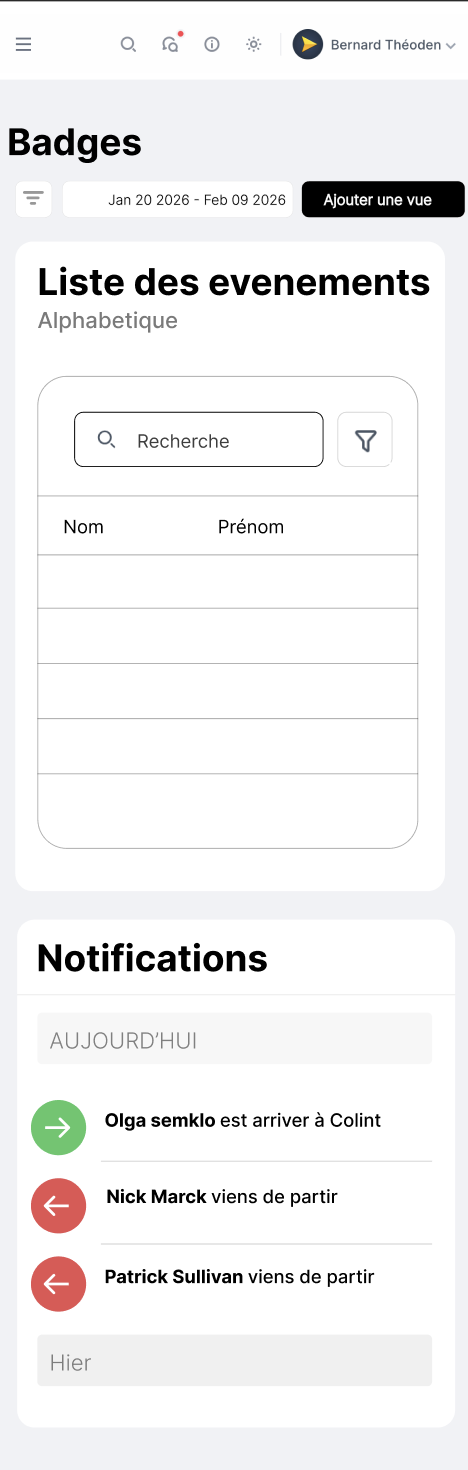
\includegraphics[height=7.2cm]{./assets/maquette/page_badge_mobile.png}
\end{for_you}

\textbf{\newline}

\begin{for_you}{Page profile}
    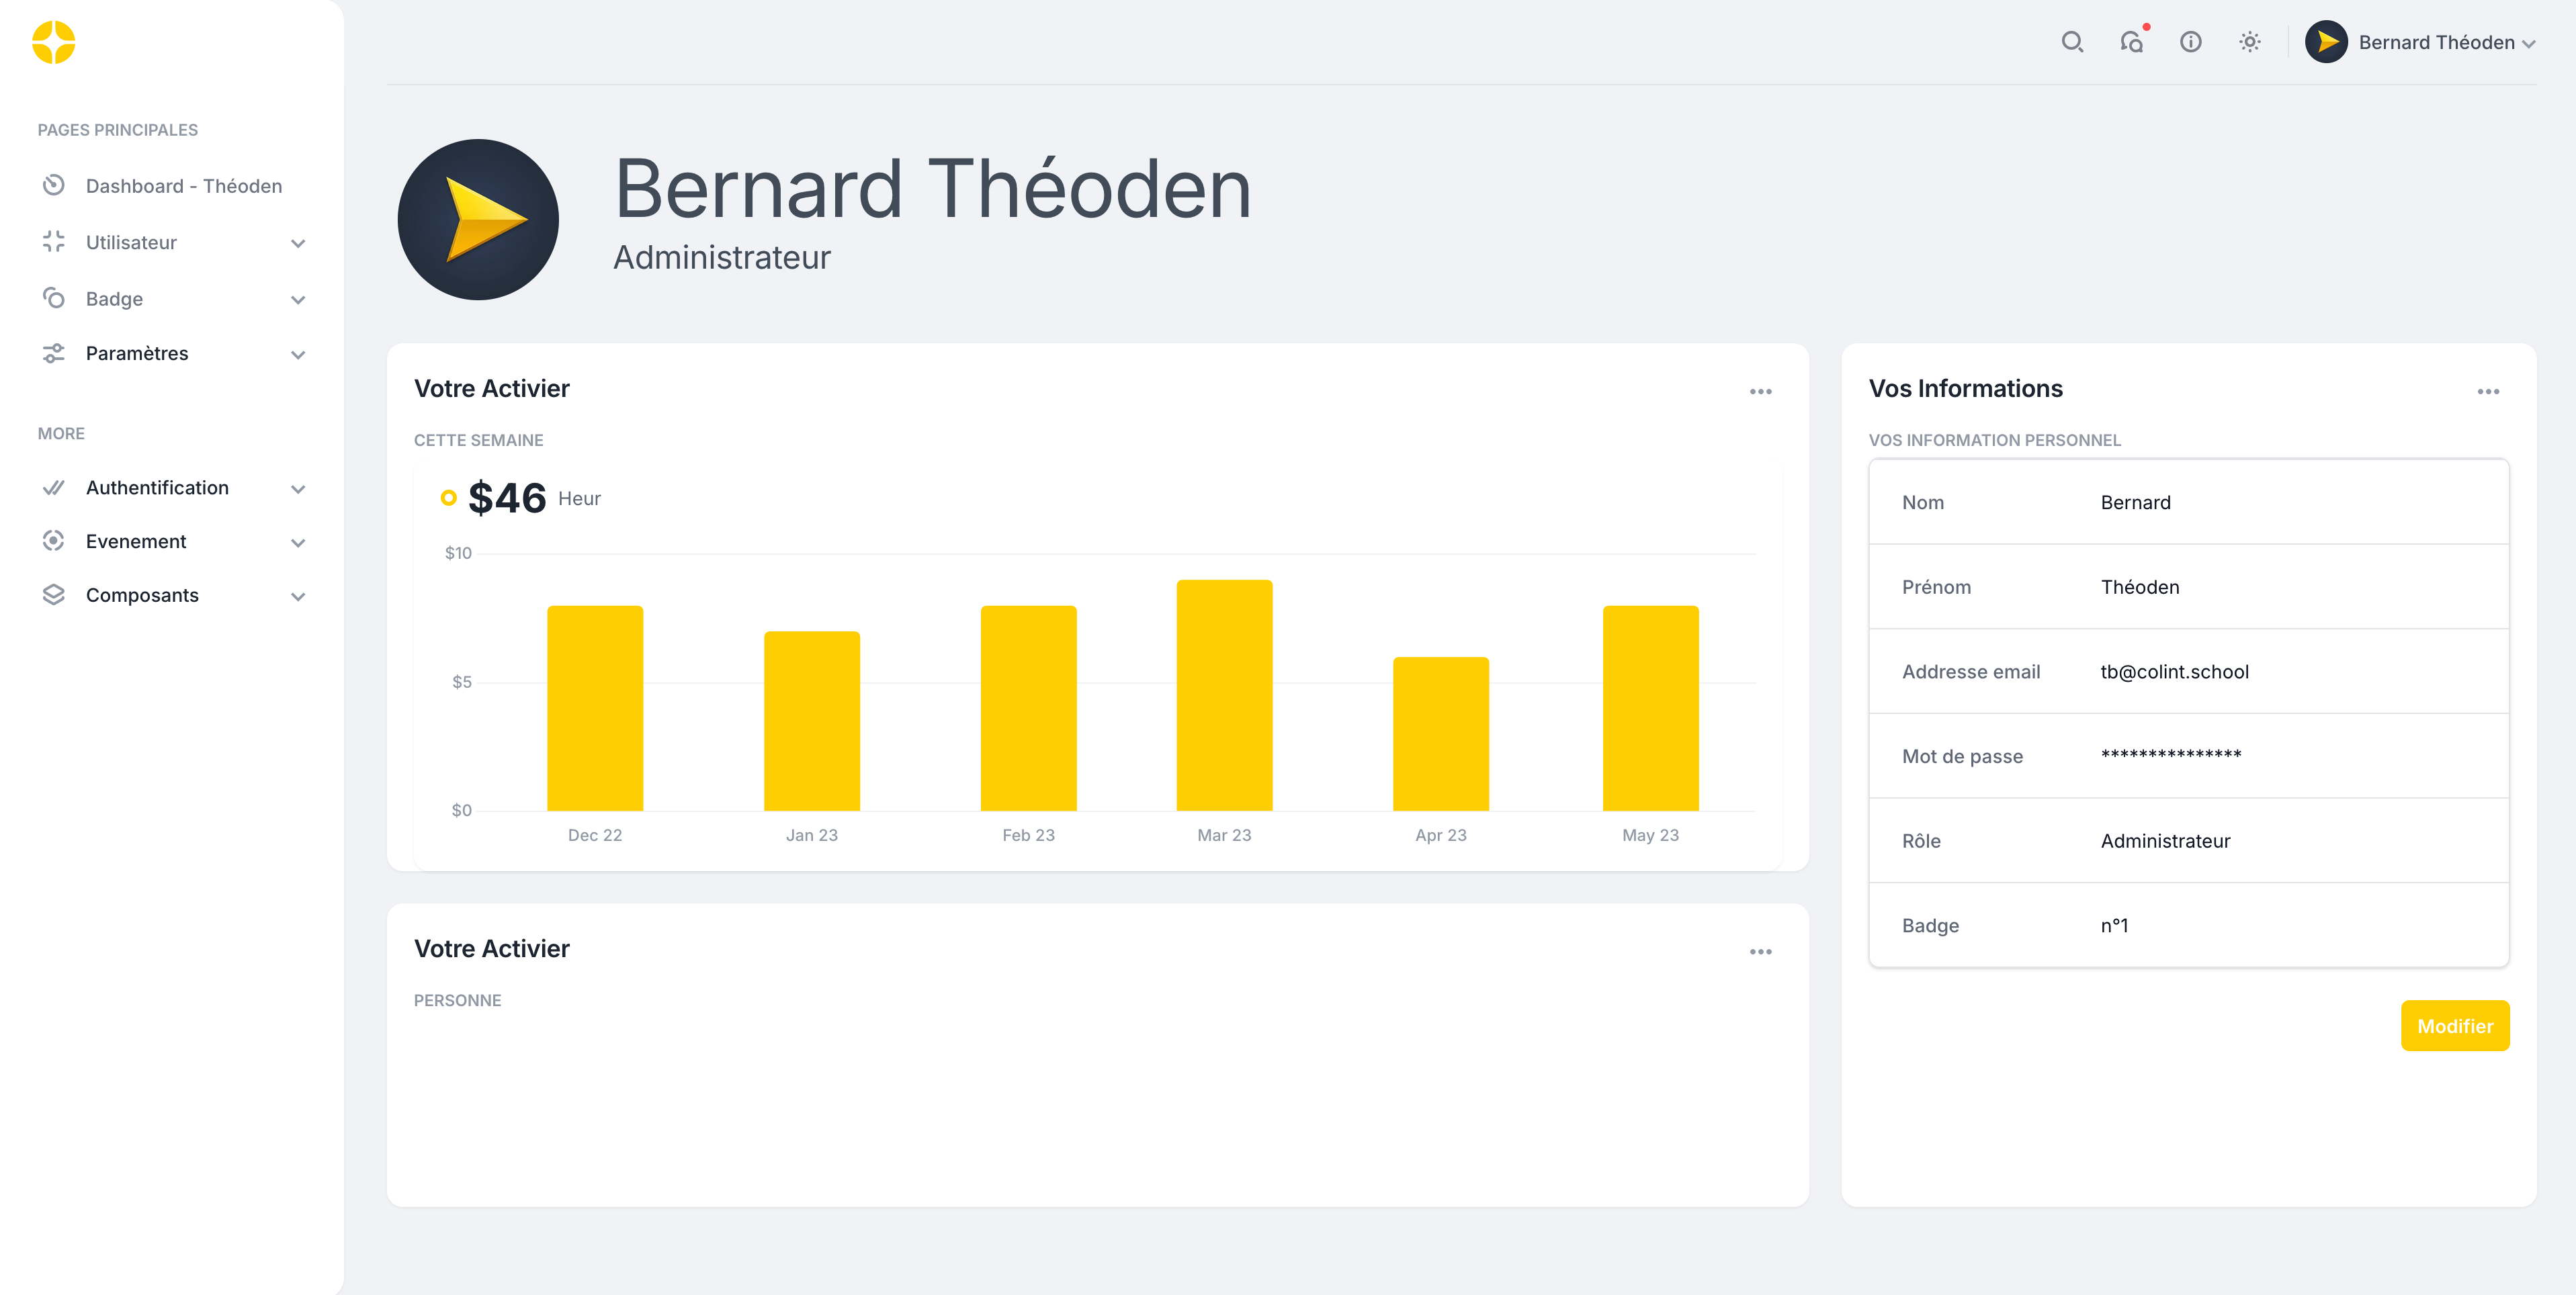
\includegraphics[height=6.5cm]{./assets/maquette/page_profile.png}
    \hfil
    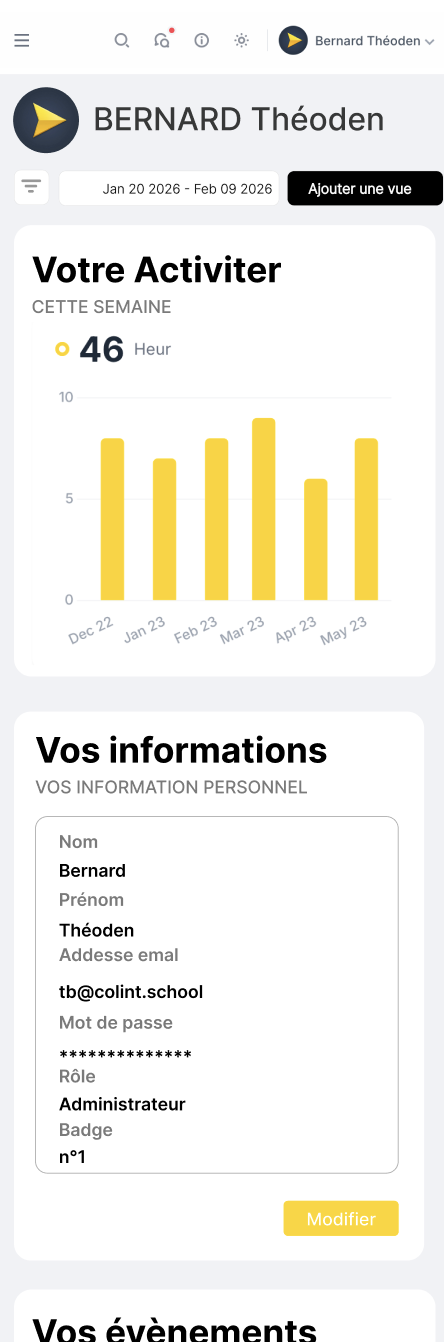
\includegraphics[height=6.5cm]{./assets/maquette/page_profile_mobile.png}
\end{for_you}

\textbf{\newline}

\begin{for_you}{Modale de création d'utilisateur}
    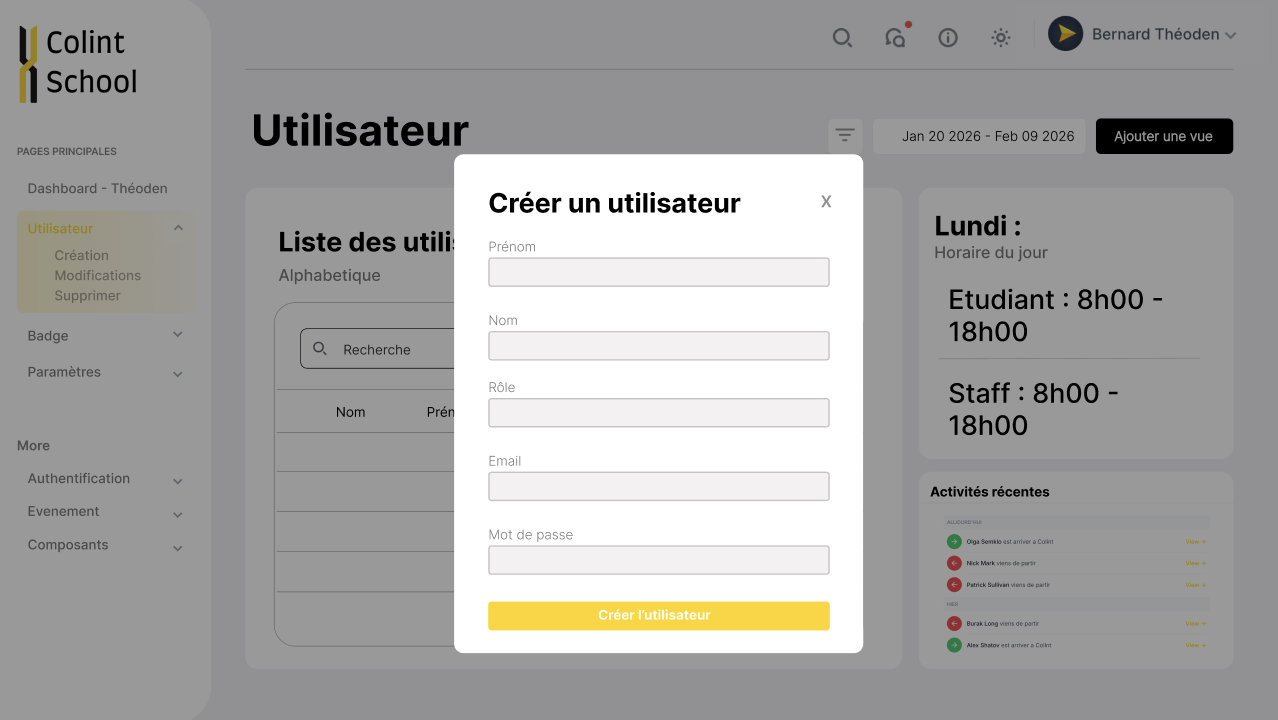
\includegraphics[height=7.2cm]{./assets/maquette/page_creation_utilisateur.png}
    \hfil
    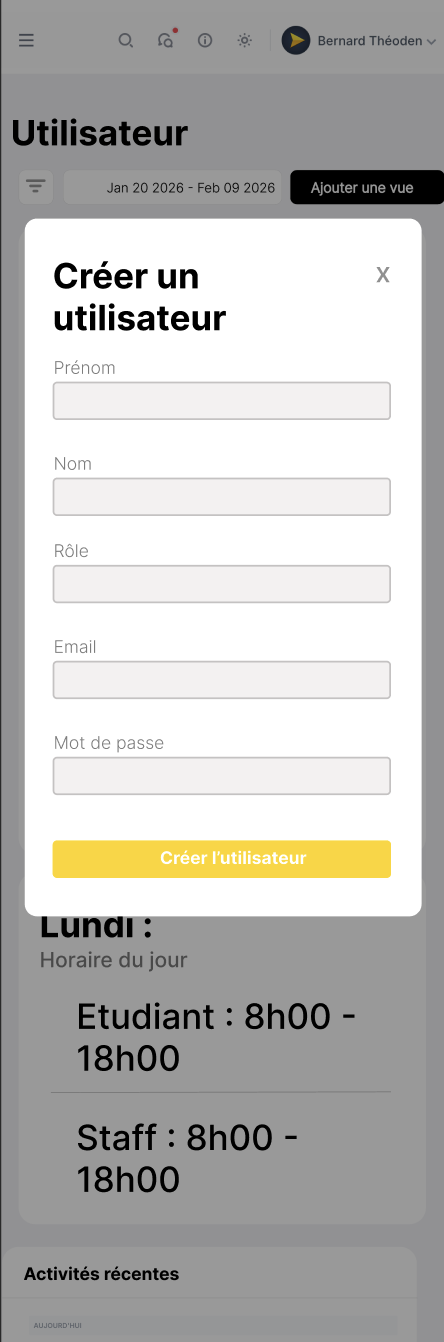
\includegraphics[height=7.2cm]{./assets/maquette/page_creation_utilisateur_mobile.png}
\end{for_you}

\section{Tableau du Dictionnaire de Données}
\hypertarget{cible:dictionnaire}{}

Ce dictionnaire de données constitue le document de référence qui m'a permis de construire mon Modèle Conceptuel de Données (MCD) et d'avoir une vue globale et précise sur tout ce dont j'avais besoin pour ma future base de données.

\begin{longtable}{p{3.5cm} p{3.5cm} c p{6.5cm}}
    \toprule
    \textbf{Nom de la donnée} & \textbf{Format} & \textbf{Longueur} & \textbf{Description} \\
    \midrule
    \endhead

    \bottomrule
    \endfoot

    \multicolumn{4}{l}{\textbf{identité : Users\_tokens}} \\
        \hline
        \texttt{id\_user\_token} & Numérique (Entier) & -- & Clé primaire auto-incrémentée \\
        \texttt{token} & Alphanumérique & 255 & Chaîne unique pour la validation du jeton \\
        \texttt{context} & Alphanumérique & 50 & Contexte du jeton (ex: "session", "activation") \\
        \texttt{sent\_to} & Alphanumérique & 255 & Email de destination du cookie \\
        \texttt{authenticated\_at} & Date/Heure (Timestamp) & -- & Date et heure de validation \\
    \midrule

    \multicolumn{4}{l}{\textbf{identité : Users}} \\
        \hline
        \texttt{id\_user} & Numérique (Entier) & -- & Clé primaire auto-incrémentée de l'utilisateur \\
        \texttt{firstname} & Alphanumérique & 100 & Prénom de l'utilisateur \\
        \texttt{lastname} & Alphanumérique & 100 & Nom de famille de l'utilisateur \\
        \texttt{email} & Alphanumérique & 255 & Adresse email unique \\
        \texttt{hashed\_password} & Alphanumérique & 255 & Empreinte sécurisée du mot de passe \\
        \texttt{confirmed\_at} & Date/Heure (Timestamp) & -- & Date de confirmation du compte \\
    \midrule

    \multicolumn{4}{l}{\textbf{identité : Badges}} \\
        \hline
        \texttt{id\_badge} & Numérique (Entier) & -- & Clé primaire auto-incrémentée du badge \\
        \texttt{rfid} & Alphanumérique & 64 & Identifiant unique physique de la puce RFID \\
        \texttt{name\_badge} & Alphanumérique & 100 & Nom ou libellé du badge \\
        \texttt{activation\_date} & Date & -- & Date de début de validité \\
        \texttt{expiration\_date} & Date & -- & Date de fin de validité \\
        \texttt{status} & Booléen & -- & État du badge (\texttt{true} = actif, \texttt{false} = inactif) \\
    \midrule

    \multicolumn{4}{l}{\textbf{identité : Roles}} \\
        \hline
        \texttt{id\_role} & Numérique (Entier) & -- & Clé primaire auto-incrémentée du rôle \\
        \texttt{name\_role} & Alphanumérique & 50 & Nom du rôle (ex: "admin", "etudiant") \\
    \midrule

    \multicolumn{4}{l}{\textbf{identité : Access\_points}} \\
        \hline
        \texttt{id\_access\_point} & Numérique (Entier) & -- & Clé primaire auto-incrémentée du point d'accès \\
        \texttt{name\_access\_point} & Alphanumérique & 100 & Nom ou emplacement du lecteur \\
        \texttt{places} & Alphanumérique & 255 & Zone géographique ou salle associée \\
    \midrule

    \multicolumn{4}{l}{\textbf{identité : Logs}} \\
        \hline
        \texttt{id\_log} & Numérique (Grand Entier) & -- & Clé primaire auto-incrémentée (type BIGINT) \\
        \texttt{type} & Alphanumérique & 50 & Type d'événement (ex: "in", "out") \\
        \texttt{clocked\_at} & Date/Heure (Timestamp) & -- & Date et heure précises du passage \\

\end{longtable}